% Title:   UofT Art & Sciences Assignment Sample File
% Version: 1.00
% Author:  Kaveh Ghasemloo
% Date:    Sept. 28, 2012
%
% Licence: 
% This work is licensed under the Creative Commons Attribution-ShareAlike 3.0 Unported License. To view a copy of this license, visit http://creativecommons.org/licenses/by-sa/3.0/ or send a letter to Creative Commons, 444 Castro Street, Suite 900, Mountain View, California, 94041, USA.

\documentclass[10pt]{csc_assignment}
\usepackage[]{algorithm2e}
\usepackage{amsmath}
\usepackage{algpseudocode}
\usepackage{qtree}
\usepackage{tkz-graph}

% ----------------------------------------------------------------
% TODO: Enter the assignment number, your name, and your student number below
% ----------------------------------------------------------------
\AssignmentName{3}
\QuestionCount{8}
\StudentName{John Armstrong, Henry Ku}
\StudentNumber{993114492\textbackslash g2jarmst, 998551348\textbackslash g2kuhenr}

% ----------------------------------------------------------------
\begin{document}


\Acknowledgements{
% ----------------------------------------------------------------
% TODO: Write your acknowledgements below.
% ----------------------------------------------------------------

"We declare that we have not used any outside help in completing this assignment."

% ----------------------------------------------------------------
% Aacknowledgements ends
% ----------------------------------------------------------------
}
\begin{description}

\newpage
\item[Q1.]
% ----------------------------------------------------------------
% TODO: Write your answer to the question below. 
% ----------------------------------------------------------------

Suppose G(V, E) is representative of a network where V = \{s, t, v$_{1}$, ..., v$_{n}$\} 
and E is the set of edges that make up this network. Suppose we have sets S and T such that
s $\in$ S, t $\in$ T, (S $\cup$ T) - \{s, t\} = V, and S $\cap$ T = $\emptyset$. Also, 
suppose that for all possible arrangement of vertices in S and T, c(S, T) = f(S, T), which means that G(V, E) has an exponential number of minimum cuts between s and t. Precisely, 2$^{n}$ minimum cuts as each vertex is either in S or T and cannot be in both, thus it is much like a binary string of $\mid$V$\mid$ elements, which can be expressed in 2$^{n}$ possible ways.\\

To construct a graph that is representative of there being 2$^{n}$ possible minimum cuts, a tree
like structure seems appropriate since there are 2$^{n}$ leaves in a full and complete tree for n levels in the tree. Taking inspiration from Huffman encoding, we wish to have a graph that for each leaf in a full tree will represent a unique binary string that represents whether a vertex is in S or T. Suppose we arrange the the string as follows, v$_{1}$, ..., v$_{n}$, where if v$_{i}$ is in S then v$_{i}$ = 0 and v$_{i}$ = 1 if it is in T. The tree/graph can be constructed so that each left edge appends 0 to the vertex string, and WLOG each right edge appends 1. Finally, when reaching any leaf we have an n length binary string that represents a unique cut S, T. In total there are 2$^{n}$ such possible cuts.\\ 

For example, suppose we had $\mid$V$\mid$ = 3 and we are certain that there are an exponential number of minimum cuts. We construct a full and complete binary tree as follows to represent the minimum cuts:\\

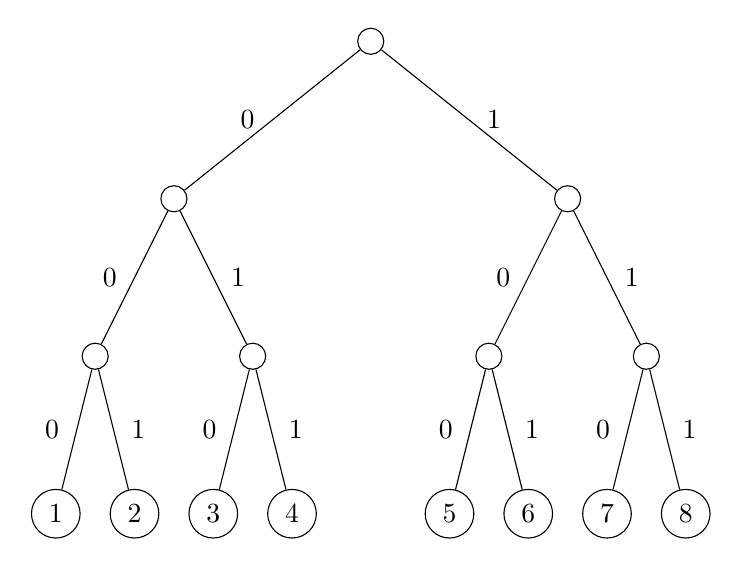
\begin{tikzpicture}[level distance=2cm,
level 1/.style={sibling distance=5cm},
level 2/.style={sibling distance=2 cm},
level 3/.style={sibling distance=1cm}]
\tikzstyle{every node}=[circle,draw]

\node (Root) {}
    child {
    node {} 
    child { node {} 
	child {  node {1} edge from parent node[left,draw=none] {0} }
    	child { node {2} edge from parent node[right,draw=none] {1} }
    	edge from parent node[left,draw=none] {0} 
    }
    child { node {} 
	child { node {3} edge from parent node[left,draw=none] {0} }
    	child { node {4} edge from parent node[right,draw=none] {1} }
	edge from parent node[right,draw=none] {1} 
    }
    edge from parent node[left,draw=none] {0}
}
child {
    node {}
    child { node {} 
	child {  node {5} edge from parent node[left,draw=none] {0} }
    	child { node {6} edge from parent node[right,draw=none] {1} }
    	edge from parent node[left,draw=none] {0} 
    }
    child { node {} 
	child {  node {7} edge from parent node[left,draw=none] {0} }
    	child { node {8} edge from parent node[right,draw=none] {1} }
	edge from parent node[right,draw=none] {1} 
    }
    edge from parent node[right,draw=none] {1}
};

\end{tikzpicture} \\

If we were to trace each leaf from the node, in a similar fashion to Huffman encoding, we would have \mbox{1: 000, 2: 001, 3: 010, 4: 011, 5: 100, 6: 101, 7: 110, and 8: 111.} So, it is clear that each binary string representing \mbox{v$_{1}$, v$_{2}$, v$_{3}$} will represent all possible sets S, T such that in total the constructed graph can represent an exponential number of minimum cuts. 

% ----------------------------------------------------------------
% Answer ends
% ----------------------------------------------------------------

\newpage
\item[Q2.]
% ----------------------------------------------------------------
% TODO: Write your answer to the question below. 
% ----------------------------------------------------------------

\textbf{Claim:}\\
Function f, such that f(S) is the number of edges (u, v) with u $\in$ S, v $\in$ V$\backslash$S, is 
submodular.\\

\textbf{Proof:}\\
Using the fact provided in the question, all that is necessary to show that f is 
submodular is to show that for any two subsets A, B $\subseteq$ V, \mbox{f(A) + 
f(B) $\geqslant$ f(A $\cup$ B) + f(A $\cap$ B)}.\\

We begin by establishing a fact. Suppose you have disjoint sets X$_{1}$, X$_{2}$, ..., X$_{k}$  $\subseteq$ V, k \textgreater ~1. \\
\underline{Case 1:} Assume that in each X$_{i}$ the set of vertices can be divided into two sets, those that exist as startpoints of edges in E and those that exist as endpoints in E. 
However, $\forall$ u $\in$ X$_{i}$, $\nexists$ v $\in$ X$_{i}$ such that (u, v) $\in$ E. It follows that f(X$_{i}$) $\geqslant$ 0. Additionally, suppose that $\forall$ u $\in$ X$_{1}$ $\cup$ X$_{2}$ $\cup$ ... $\cup$ X$_{k}$, $\exists$ v $\in$ X$_{1}$ $\cup$ X$_{2}$ $\cup$ ... $\cup$  X$_{k}$, such that (u, v) $\in$ E. It follows that f(X$_{1}$ $\cup$ X$_{2}$ $\cup$ ... $\cup$  X$_{k}$) = 0, and so \mbox{f(X$_{1}$) + f(X$_{2}$) + ... + f(X$_{k}$) $\geqslant$ f(X$_{1}$ $\cup$ X$_{2}$ $\cup$ ... $\cup$  X$_{k}$).}\\
\underline{Case 2:} Assume that $\forall$ u $\in$ X$_{i}$ $\nexists$ v $\in$ X$_{j}$, such that (u, v) $\in$ E. Also, i $\neq$ j and 1 $\geqslant$ i, j $\geqslant$ k. So, it would follow that \mbox{f(X$_{1}$) + f(X$_{2}$) + ... + f(X$_{k}$)} = \mbox{f(X$_{1}$ $\cup$ X$_{2}$ $\cup$ ... $\cup$  X$_{k}$).}\\ 

Both Case 1 and Case 2 represent the least ideal and most ideal cases, respectively. It follows that in all cases the function f on the union of any series of disjoint subsets of V will result in a value less than or equal to the summation of values of f operating on each subset seperately, thus, \mbox{f(X$_{1}$) + f(X$_{2}$) + ... + f(X$_{k}$) $\geqslant$ f(X$_{1}$ $\cup$ X$_{2}$ $\cup$ ... $\cup$  X$_{k}$).}\\

Now, suppose we have some arbitrary subsets A, B $\subseteq$ V. Indeed, it is possible to seperate both A and B as follows. Let A' represent all vertices from A that do not appear in B, and conversely let A'' be those vertices that do appear in both A and B. Similarly, Let B' represent all vertices from B that do not appear in A, and let B'' be those vertices that appear in A and B. Then, \mbox{f(A) + f(B) = f(A') + f(A'') + f(B') + f(B'')}. Clearly, \mbox{A'' = B'' = (A $\cap$ B)}, then \mbox{f(A) + f(B) = (f(A') + f(A $\cap$ B) + f(B')) + f(A $\cap$ B)}. It follows by our construction of A' and B' that the sets A', (A $\cap$ B), and B' are disjoint. Then using the fact proven above, \mbox{(f(A') + f(A $\cap$ B) + f(B')) $\geqslant$ f(A' $\cup$ (A $\cap$ B) $\cup$ B').} However, \mbox{(A' $\cup$ (A $\cap$ B) $\cup$ B') = (A $\cup$ B)}. Finally, \\f(A) + f(B) = (f(A') + f(A $\cap$ B) + f(B')) + f(A $\cap$ B) $\geqslant$ f(A $\cup$ B) + f(A $\cap$ B). \\

Indeed, \mbox{f(A) + f(B) $\geqslant$ f(A $\cup$ B) + f(A $\cap$ B)} implies that function f,
such that f(S) is the number of edges \mbox{(u, v)} with u $\in$ S, v $\in$ V$\backslash$S, is 
submodular, by the equivalence of submodular functions.
 

% ----------------------------------------------------------------
% Answer ends
% ----------------------------------------------------------------

\newpage
\item[Q3.]
% ----------------------------------------------------------------
% TODO: Write your answer to the question below. 
% ----------------------------------------------------------------

% ----------------------------------------------------------------
% Answer ends
% ----------------------------------------------------------------

\newpage
\item[Q4.]
% ----------------------------------------------------------------
% TODO: Write your answer to the question below. 
% ----------------------------------------------------------------
    
% ----------------------------------------------------------------
% Answer ends
% ----------------------------------------------------------------

\newpage
\item[Q5.]
% ----------------------------------------------------------------                                                                               
% TODO: Write your answer to the question below.                                                                                                 
% ----------------------------------------------------------------                                                                               

% ----------------------------------------------------------------                                                                               
% Answer ends                                                                                                                                    
% ---------------------------------------------------------------- 


\newpage
\item[Q6.]
% ----------------------------------------------------------------                                                                               
% TODO: Write your answer to the question below.                                                                                                 
% ----------------------------------------------------------------                                                                               

% ----------------------------------------------------------------                                                                               
% Answer ends                                                                                                                                    
% ----------------------------------------------------------------


\newpage
\item[Q7.]
% ----------------------------------------------------------------                                                                               
% TODO: Write your answer to the question below.                                                                                                 
% ----------------------------------------------------------------                                                                               

% ----------------------------------------------------------------                                                                               
% Answer ends                                                                                                                                    
% ----------------------------------------------------------------


\newpage
\item[Q8.]
% ----------------------------------------------------------------                                                                               
% TODO: Write your answer to the question below.                                                                                                 
% ----------------------------------------------------------------                                                                               

% ----------------------------------------------------------------                                                                               
% Answer ends                                                                                                                                    
% ----------------------------------------------------------------
\end{description}
\end{document}
